\chapter{Introduction}
% \chapter{Einleitung}
\label{ch:introduction}

\pagenumbering{arabic}
\setcounter{page}{1}


\section{Background}
\label{subsec:background}

Example reference to \autoref{fig:neural_network}, which is based on \cite{kim2017neural}.

\begin{figure}[!h]
	\centering 
	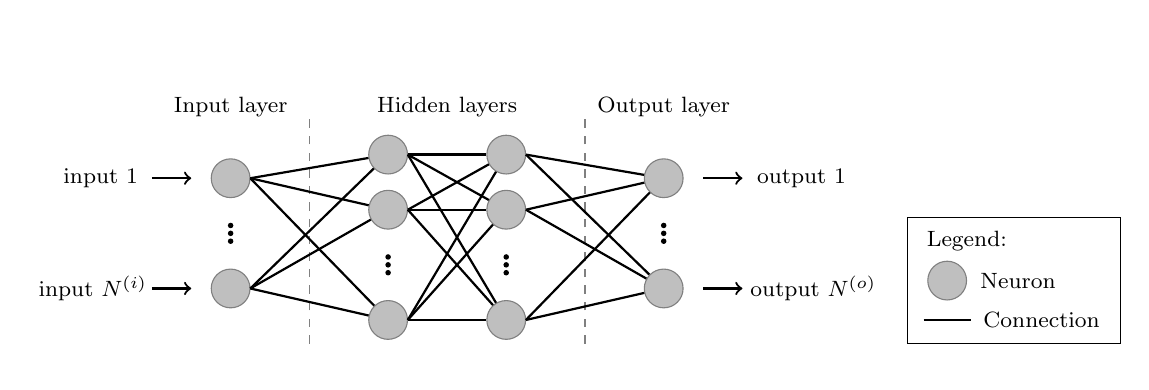
\begin{tikzpicture}
		\begin{footnotesize}			
			\node[circle, align=center] at (-1.65,1.8) () {input 1};
			\draw[black, thick, ->] (-1,1.8)--(-0.5,1.8);
			\node[circle, align=center] at (-1.75,0.4) () {input $N^{(i)}$};
			\draw[black, thick, ->] (-1,0.4)--(-0.5,0.4);			
			\node[circle, align=center] at (0,2.7) () {Input layer};
			\node[circle, draw=gray, fill=lightgray, minimum size=14pt, align=center]
			at (0,1.8) (i1) {};
			\node[circle, fill=black, inner sep=0pt, minimum size=2pt, align=center]
			at (0,1.2) () {};
			\node[circle, fill=black, inner sep=0pt, minimum size=2pt, align=center]
			at (0,1.1) () {};
			\node[circle, fill=black, inner sep=0pt, minimum size=2pt, align=center]
			at (0,1) () {};
			\node[circle, draw=gray, fill=lightgray, minimum size=14pt, align=center]
			at (0,0.4) (i2) {};			
			\draw[gray, dashed] (1,-0.3)--(1,2.6);			
			\node[circle, align=center] at (2.75,2.7) () {Hidden layers};
			\node[circle, draw=gray, fill=lightgray, minimum size=14pt, align=center]
			at (2,2.1) (h11) {};
			\node[circle, draw=gray, fill=lightgray, minimum size=14pt, align=center]
			at (2,1.4) (h12) {};
			\node[circle, fill=black, inner sep=0pt, minimum size=2pt, align=center]
			at (2,0.8) () {};
			\node[circle, fill=black, inner sep=0pt, minimum size=2pt, align=center]
			at (2,0.7) () {};
			\node[circle, fill=black, inner sep=0pt, minimum size=2pt, align=center]
			at (2,0.6) () {};
			\node[circle, draw=gray, fill=lightgray, minimum size=14pt, align=center]
			at (2,0) (h13) {};			
			\node[circle, draw=gray, fill=lightgray, minimum size=14pt, align=center]
			at (3.5,2.1) (h21) {};
			\node[circle, draw=gray, fill=lightgray, minimum size=14pt, align=center]
			at (3.5,1.4) (h22) {};
			\node[circle, fill=black, inner sep=0pt, minimum size=2pt, align=center]
			at (3.5,0.8) () {};
			\node[circle, fill=black, inner sep=0pt, minimum size=2pt, align=center]
			at (3.5,0.7) () {};
			\node[circle, fill=black, inner sep=0pt, minimum size=2pt, align=center]
			at (3.5,0.6) () {};
			\node[circle, draw=gray, fill=lightgray, minimum size=14pt, align=center]
			at (3.5,0) (h23) {};
			
			\draw[gray, dashed] (4.5,-0.3)--(4.5,2.6);
			
			\node[circle, align=center] at (5.5,2.7) () {Output layer};
			\node[circle, draw=gray, fill=lightgray, minimum size=14pt, align=center]
			at (5.5,1.8) (o1) {};
			\node[circle, fill=black, inner sep=0pt, minimum size=2pt, align=center]
			at (5.5,1.2) () {};
			\node[circle, fill=black, inner sep=0pt, minimum size=2pt, align=center]
			at (5.5,1.1) () {};
			\node[circle, fill=black, inner sep=0pt, minimum size=2pt, align=center]
			at (5.5,1) () {};
			\node[circle, draw=gray, fill=lightgray, minimum size=14pt, align=center]
			at (5.5,0.4) (o2) {};
			
			\node[circle, align=center] at (7.25,1.8) () {output 1};
			\draw[black, thick, ->] (6,1.8)--(6.5,1.8);
			\node[circle, align=center] at (7.4,0.4) () {output $N^{(o)}$};
			\draw[black, thick, ->] (6,0.4)--(6.5,0.4);	
			
			\draw[black, thick, -] (0.25,1.8) -- (h11);
			\draw[black, thick, -] (0.25,1.8) -- (h12);
			\draw[black, thick, -] (0.25,1.8) -- (h13);
			\draw[black, thick, -] (0.25,0.4) -- (h11);
			\draw[black, thick, -] (0.25,0.4) -- (h12);
			\draw[black, thick, -] (0.25,0.4) -- (h13);
			
			\draw[black, thick, -] (2.25,2.1) -- (h21);
			\draw[black, thick, -] (2.25,2.1) -- (h22);
			\draw[black, thick, -] (2.25,2.1) -- (h23);
			\draw[black, thick, -] (2.25,1.4) -- (h21);
			\draw[black, thick, -] (2.25,1.4) -- (h22);
			\draw[black, thick, -] (2.25,1.4) -- (h23);
			\draw[black, thick, -] (2.25,0) -- (h21);
			\draw[black, thick, -] (2.25,0) -- (h22);
			\draw[black, thick, -] (2.25,0) -- (h23);
			
			\draw[black, thick, -] (3.75,2.1) -- (o1);
			\draw[black, thick, -] (3.75,2.1) -- (o2);
			\draw[black, thick, -] (3.75,1.4) -- (o1);
			\draw[black, thick, -] (3.75,1.4) -- (o2);
			\draw[black, thick, -] (3.75,0) -- (o1);
			\draw[black, thick, -] (3.75,0) -- (o2);
			
			\draw[draw=black] (8.6,-0.3) rectangle ++(2.7,1.6);
			\node[rectangle, align=center] at (9.35,1) () {Legend:};
			\node[circle, draw=gray, fill=lightgray, minimum size=14pt, align=center]
			at (9.1,0.5) (neuron) {};
			\node[rectangle, align=center] at (10,0.5) () {Neuron};
			\draw[black, thick, -] (8.8, 0) -- (9.4, 0);
			\node[rectangle, align=center] at (10.3,0) () {Connection};
		\end{footnotesize}
	\end{tikzpicture}
	\caption[Structure of a neural network]{Structure of a neural network.}
	\label{fig:neural_network}
\end{figure}

\section{Something Location}
\label{subsec:somelocation}

write here

See more in~\autoref{subsec:background}
write here
	
\begin{center}
\end{center}
